\documentclass[a4paper,oneside,14pt]{extreport}

% ==================================================
% Кодировки и языки (bmstu.cls)
% ==================================================
\usepackage{cmap}
\usepackage[OT2,T2C,T2B,T2A,LGR,T1]{fontenc}
\usepackage[utf8]{inputenc}
\usepackage[english,main=russian]{babel}
\usepackage{tempora}
\usepackage[scaled=0.95]{PTMono}

% ==================================================
% Геометрия страницы (bmstu.cls)
% ==================================================
\usepackage[
left=30mm,
right=15mm,
top=20mm,
bottom=20mm,
]{geometry}

% ==================================================
% Типографика и переносы
% ==================================================
\usepackage[expansion=false]{microtype}
\sloppy
\hyphenpenalty=50
\exhyphenpenalty=50

% ==================================================
% Межстрочный интервал
% ==================================================
\usepackage{setspace}
\onehalfspacing

% ==================================================
% Абзацы
% ==================================================
\usepackage{indentfirst}
\setlength{\parindent}{12.5mm}

% ==================================================
% Размеры шрифтов заголовков
% ==================================================
\makeatletter
\renewcommand\LARGE{\@setfontsize\LARGE{22pt}{20}}
\renewcommand\Large{\@setfontsize\Large{20pt}{20}}
\renewcommand\large{\@setfontsize\large{16pt}{20}}
\makeatother

% ==================================================
% Заголовки
% ==================================================
\usepackage{titlesec}

\titleformat{\chapter}[block]
{\hspace{\parindent}\large\bfseries}
{\thechapter}{0.5em}{\large\bfseries\raggedright}

\titleformat{name=\chapter,numberless}[block]
{\hspace{\parindent}}{}{0pt}{\large\bfseries\centering}

\titleformat{\section}[block]
{\hspace{\parindent}\large\bfseries}
{\thesection}{0.5em}{\large\bfseries\raggedright}

\titleformat{\subsection}[block]
{\hspace{\parindent}\large\bfseries}
{\thesubsection}{0.5em}{\large\bfseries\raggedright}

\titleformat{\subsubsection}[block]
{\hspace{\parindent}\large\bfseries}
{\thesubsubsection}{0.5em}{\large\bfseries\raggedright}

\titlespacing{\chapter}{12.5mm}{-22pt}{10pt}
\titlespacing{\section}{12.5mm}{10pt}{10pt}
\titlespacing{\subsection}{12.5mm}{10pt}{10pt}
\titlespacing{\subsubsection}{12.5mm}{10pt}{10pt}

% ==================================================
% Цвета
% ==================================================
\usepackage{xcolor,colortbl}

% ==================================================
% Таблицы и окружения (твои пакеты)
% ==================================================
\usepackage{tabularx}
\usepackage{tabulary}
\usepackage{threeparttable}
\usepackage{multirow}
\usepackage{booktabs}
\usepackage{pgfplots}
\pgfplotsset{compat=1.18}

% ==================================================
% Подписи
% ==================================================
\usepackage{caption}
\captionsetup{
	labelsep=endash,
	figurename=Рисунок,
	singlelinecheck=false,
}

\captionsetup[figure]{justification=centering}

\captionsetup[table]{
	justification=centering,
	singlelinecheck=false,
	position=above,
	skip=6pt
}

% ==================================================
% Повороты и альбомные страницы
% ==================================================
\usepackage{rotating}
\usepackage{lscape}
\usepackage{pdflscape}
\usepackage{afterpage}

% ==================================================
% Математика
% ==================================================
\usepackage{amsmath}
\usepackage{amssymb}

% ==================================================
% Библиография (bmstu.cls)
% ==================================================
\usepackage[
backend=biber,
style=gost-numeric,
language=auto,
autolang=other,
sorting=none,
]{biblatex}

\addbibresource{biblio.bib}

\usepackage{csquotes}

\DeclareFieldFormat{urldate}
{(Дата обращения:\addspace\ifnum\thefield{urlday}<10 0\fi\thefield{urlday}\adddot\ifnum\thefield{urlmonth}<10 0\fi\thefield{urlmonth}\adddot\thefield{urlyear})}
\DeclareFieldFormat[online]{title}{#1\addspace\mkbibbrackets{Электронный ресурс}}
\DeclareFieldFormat{url}{Режим доступа URL\addcolon\space\url{#1}}

% ==================================================
% Гиперссылки
% ==================================================
\usepackage[unicode,hidelinks]{hyperref}

% ==================================================
% Управляющие пакеты
% ==================================================
\usepackage{xifthen}
\usepackage{etoolbox}
\usepackage{totcount}
\usepackage{assoccnt}
\usepackage{placeins}
\usepackage{changepage}
\usepackage{pdfpages}
\usepackage{needspace}
%\usepackage{soul}
%\usepackage{svg}
%\usepackage{shellesc}

% ==================================================
% Содержание (bmstu-toc)
% ==================================================
\newcommand{\maketableofcontents}{
	\renewcommand\contentsname{СОДЕРЖАНИЕ}
	\tableofcontents
}

\setcounter{secnumdepth}{3}
\setcounter{tocdepth}{2}

% ==================================================
% Счётчики рисунков, таблиц, источников (bmstu-essay)
% ==================================================
\usepackage{lastpage}

\newcounter{totfigures}
\newcounter{tottables}
\providecommand\totfig{}
\providecommand\tottab{}

\makeatletter
\AtEndDocument{
	\addtocounter{totfigures}{\value{figure}}
	\addtocounter{tottables}{\value{table}}
	\immediate\write\@mainaux{
		\string\gdef\string\totfig{\number\value{totfigures}}
		\string\gdef\string\tottab{\number\value{tottables}}
	}
}
\makeatother

\pretocmd{\chapter}{\addtocounter{totfigures}{\value{figure}}\setcounter{figure}{0}}{}{}
\pretocmd{\chapter}{\addtocounter{tottables}{\value{table}}\setcounter{table}{0}}{}{}
\pretocmd{\section}{\Needspace{8\baselineskip}}{}{}
\pretocmd{\subsection}{\Needspace{7\baselineskip}}{}{}
\pretocmd{\subsubsection}{\Needspace{6\baselineskip}}{}{}

% ==================================================
% Подсчёт источников
% ==================================================
\newcounter{totbibentries}
\newcommand*{\listcounted}{}

\makeatletter
\AtDataInput{
	\xifinlist{\abx@field@entrykey}\listcounted
	{}
	{\stepcounter{totbibentries}
		\listxadd\listcounted{\abx@field@entrykey}}
}
\makeatother

% ==================================================
% Приложения (bmstu-appendix)
% ==================================================
\usepackage[titletoc,title]{appendix}
\usepackage{titlesec}

\AtBeginDocument{\renewcommand{\appendixname}{ПРИЛОЖЕНИЕ}}

\let\oldappendices\appendices
\let\oldendappendices\endappendices

% Новое окружение appendices с опциональным аргументом для буквы
\usepackage{xparse}
\RenewDocumentEnvironment{appendices}{o} % o = optional argument
{
	\titleformat{\chapter}{\large\bfseries}
	{\appendixname~\IfValueTF{#1}{#1}{\thechapter}}{0pt}
	{\centering\large\bfseries\\}
	\oldappendices
	% если передали букву, используем её для визуала и PDF bookmarks
	\IfValueTF{#1}{
		\renewcommand{\thechapter}{#1}
	}{
		\renewcommand{\thechapter}{\Asbuk{chapter}} % кириллическая нумерация по умолчанию
	}
}
{
	\oldendappendices
}
% ==================================================
% Определения и сокращения (твоя версия)
% ==================================================
\usepackage{enumitem}

\newcommand{\mydefinition}[2]{
	\item \noindent #1 --- #2
}

\newenvironment{mydefinitions}{
	\chapter*{ОПРЕДЕЛЕНИЯ}
	\addcontentsline{toc}{chapter}{ОПРЕДЕЛЕНИЯ}
	\begin{description}[leftmargin=0pt]
	}{
	\end{description}
}

\newenvironment{myabbreviations}{
	\chapter*{ОБОЗНАЧЕНИЯ И СОКРАЩЕНИЯ}
	\addcontentsline{toc}{chapter}{ОБОЗНАЧЕНИЯ И СОКРАЩЕНИЯ}
	\begin{description}[leftmargin=0pt]
	}{
	\end{description}
}

% ==================================================
% TOC: оформление глав (твой патч)
% ==================================================
\makeatletter
\renewcommand*{\l@chapter}[2]{
	\ifnum \c@tocdepth>\m@ne
	\addpenalty{-\@highpenalty}
	\vskip 1em \@plus.2em
	\@dottedtocline{0}{0pt}{1.5em}{\bfseries #1}{\bfseries #2}
	\fi
}
\makeatother


\newenvironment{essay}[1]
{
	\clearpage
	\chapter*{РЕФЕРАТ}
	\addcontentsline{toc}{chapter}{РЕФЕРАТ}
	
	% --- строка с подсчётами (безопасно, если приложений ещё нет)
	Расчётно-пояснительная записка \begin{NoHyper}\pageref{LastPage}\end{NoHyper}~с., 
	\totfig~рис., \tottab~табл., \arabic{totbibentries}~источн., 2~прил.
	
	\noindent\MakeUppercase{#1} \par
}
{
	%\vspace{1em}
	\clearpage
}

% ==================================================
% Пользовательские команды
% ==================================================
\newcommand*{\rom}[1]{\uppercase\expandafter{\romannumeral #1\relax}}

\newenvironment{formulaexplanation}
{
	\par\noindent где
	\begin{itemize}[label=---, itemsep=0pt, parsep=0pt, topsep=0pt]
}
{
	\end{itemize}
}


\bibliography{biblio}

\begin{document}
	\IfFileExists{vkr_title.pdf}{
		\includepdf[pages=-]{vkr_title.pdf}
	}{
		\null
		\thispagestyle{empty}
		\clearpage
	}
	\setcounter{page}{3}
	\begin{essay}{КЛАССИФИКАЦИЯ ИЗОБРАЖЕНИЙ, РАСПОЗНАВАНИЕ РАСТЕНИЙ, ТОНКОЗЕРНИСТАЯ КЛАССИФИКАЦИЯ, МАШИННОЕ ОБУЧЕНИЕ, СВЁРТОЧНЫЕ НЕЙРОННЫЕ СЕТИ.}
Цель работы~---~разработка метода классификации растений по изображениям листьев с использованием свёрточной нейронной сети.

В работе выполнен анализ предметной области классификации изображений растений, формализована задача классификации изображений листьев растений средней полосы России, разработан и реализован двухэтапный метод классификации с использованием свёрточной нейронной сети. Также проведено сравнение результатов работы разработанного метода с результатами классификации после прямого обучения.
\end{essay}

	\maketableofcontents

	\begin{mydefinitions}
	\mydefinition{Датасет}{набор данных, предназначенный для обучения, валидации и/или тестирования моделей машинного обучения.}
	\mydefinition{Дескриптор изображения}{вектор признаков, вычисленный по изображению и характеризующий его свойства.}
	\mydefinition{Извлечение признаков}{процесс преобразования исходного изображения в набор информативных признаков, используемых для последующей классификации.}
	\mydefinition{Классификация изображений}{задача отнесения изображения к одному из заранее заданных классов на основе вычисленных признаков или представлений, полученных моделью.}
	\mydefinition{Модель машинного обучения}{алгоритм, параметры которого определяются в процессе обучения по данным и используются для построения прогнозов.}
	\mydefinition{Признак}{измеримая характеристика объекта, используемая для различения классов.}
	\mydefinition{Свёрточная нейронная сеть}{нейронная сеть, использующая свёрточные слои для автоматического извлечения признаков из изображений.}
	\mydefinition{Тонкозернистая классификация изображений}{классификация объектов с малозаметными межклассовыми отличиями.}
\end{mydefinitions}

	\begin{myabbreviations}
	\mydefinition{CCM}{Color Co-occurrence Matrix, матрица совместной встречаемости цветов.}
		\mydefinition{CNN}{Convolutional Neural Network, свёрточная нейронная сеть.}
	\mydefinition{FGIC}{Fine-Grained Image Classification, тонкозернистая классификация изображений.}
	\mydefinition{GLCM}{Gray Level Co-occurrence Matrix, матрица совместной встречаемости уровней серого.}
	\mydefinition{HOG}{Histogram of Oriented Gradients, гистограмма ориентированных градиентов.}
	\mydefinition{ILSVRC}{ImageNet Large Scale Visual Recognition Challenge, конкурс по распознаванию изображений.}
	\mydefinition{kNN}{k-Nearest Neighbors, метод $k$ ближайших соседей.}
	\mydefinition{LBP}{Local Binary Pattern, локальные бинарные паттерны.}
	\mydefinition{ReLU}{Rectified Linear Unit, функция активации вида $\max(0, x)$.}
		\mydefinition{SCNN}{Siamese Convolutional Neural Network, сиамская свёрточная нейронная сеть.}
	\mydefinition{SGLDM}{Spatial Gray Level Dependence Matrix, матрица пространственной зависимости уровней серого.}
	\mydefinition{SVM}{Support Vector Machine, метод опорных векторов.}
\end{myabbreviations}


	\chapter*{ВВЕДЕНИЕ}
\addcontentsline{toc}{chapter}{ВВЕДЕНИЕ}

Растения имеют основополагающее значение для экосистем Земли и жизни человека, играя незаменимую роль в поддержании и улучшении глобального экологического баланса. Методы распознавания образов и обработки изображений используются для автоматизации классификации растений, что позволяет снизить трудоёмкость определения вида и расширить возможности анализа ботанических данных~\cite{ref1101}.

Цель работы~---~разработать метод классификации растений по изображениям листьев с использованием свёрточной нейронной сети.

Для достижения поставленной цели требуется решить следующие задачи:
\begin{itemize}[label=---, itemsep=0pt, parsep=0pt, topsep=0pt]
	\item провести анализ предметной области классификации изображений растений;
	\item формализовать задачу классификации изображений растений;
	\item разработать метод классификации растений по изображениям листьев с использованием свёрточной нейронной сети;
	\item сравнить разработанный метод с существующими методами.
\end{itemize}

\clearpage

	\chapter{Анализ предметной области}
\section{Классификация изображений растений}
Королевские ботанические сады в Кью опубликовали Всемирный список сосудистых растений, в котором задокументировано 350 386 признанных видов сосудистых растений~\cite{ref1102}. Автоматизация классификации такого огромного множества видов~---~сложная задача, которая стала возможной благодаря машинному обучению и методам компьютерного зрения.

Классическая задача идентификации растений основана на ручной работе специалистов-таксономистов и требует значительных временных и экспертных ресурсов. С увеличением количества доступных визуальных данных растёт потребность в автоматизированной классификации растений~\cite{ref1101}. 

\section{Особенности визуальных данных}
 Незначительные различия в форме, текстуре или цвете листьев могут разделять близкородственные виды. Сложность классификации усугубляется внешними факторами, такими как различия в фоне, позе и освещении, которые приводят к значительным различиям внутри классов изображений~\cite{ref1103}. Эта проблема решается за счёт извлечения дискриминационных признаков, которые минимизируют внутриклассовые различия и максимально увеличивают межклассовые различия.
 
Традиционно для классификации растений анализируют изображения листьев, выделяя множество признаков, таких как текстура листьев, их форма и цвет. Цветовая характеристика в большей степени зависит от классификации и идентификации видов растений, поскольку цвет листьев может меняться в зависимости от окружающей среды в разные сезоны. Характеристики текстуры в большей степени основаны на информации, полученной из его жилок и жилковании. В последнее время узоры жилок листьев считаются важным фактором для идентификации видов растений, при этом существует лишь несколько методов извлечения структуры жилок листьев~\cite{ref1101}. 

Помимо проблемы разнообразия видов и подвидов растений существует проблема количества имеющихся данных. Например, на наборе PlantCLEF 2019, сосредоточенном на тропических регионах с недостаточным количеством данных, лучшее решение имеет всего 41\% точности~\cite{ref1104} по сравнению с
96\% точностью в наборах данных по флоре умеренного пояса~\cite{ref1105}

	\chapter{Формализация задачи}
\section{Описание задачи}
Задачи классификации изображений растений заключается в определении вида или подвида растения по его изображению. Несмотря на то, что существуют различные решения задачи, можно выделить общий подход, который состоит из 4 этапов, приведённых на изображении~\ref{general}: захват изображения, предобработка изображений, извлечение признаков, использование методов классификации.

Для захвата изображения используются цифровые камеры с целью получения 2D представления, однако при решении задачи классификации могут быть использованы и менее распространённые средства, такие как тепловизионная камера, например, для сбора 2D-изображений апельсинов~\cite{ref12} и лазерный сканер для получения 3D-изображений, когда необходима полная информация о растении, как в статье "Классификация органов растений на основе поверхностных характеристик из трёхмерных облаков точек, полученных с помощью лазерного сканирования, для
фенотипирования растений"~\cite{ref15}.

Этап предобработки изображений включает в себя следующие шаги: переориентация изображения, кадрирование изображения, преобразование изображения в оттенки серого, после чего выполняется преобразование в двоичное изображение, удаление шума, растяжение контраста и инверсия порогового значения~\cite{ref19}. Исследование в~\cite{ref20} показало, что для извлечения особенностей листьев изображение листа делится на 2/4 части, а не извлекается целиком.

Этап извлечения признаков изображения имеет ключевое значение в задаче классификации, поскольку именно на основе полученных признаков модель будет принимать решение в пользу того или иного класса. Для извлечения текстурных признаков используются некоторые статистические меры, такие как матрица совместного появления цветов (CCM), матрица пространственной зависимости от уровня серого (SGLDM), матрица совместного появления уровней серого (GLCM), локальные бинарные паттерны (LBP). Существующие системы и методы распознавания растений зависят от цвета, размера, формы и текстуры изображения листа.

Этап классификации представляет собой методы, с помощью которых и определяется класс объекта на изображении. Нередко встаёт задача о подборе оптимальной пары - метода извлечения признаков и классификации. 

В рамках данной работы основное внимание уделено именно методам извлечения признаков и классификации. Этап захвата изображений не рассматривается в виду использования датасета, описанного в ограничениях.

\begin{figure}[h]
	\centering
	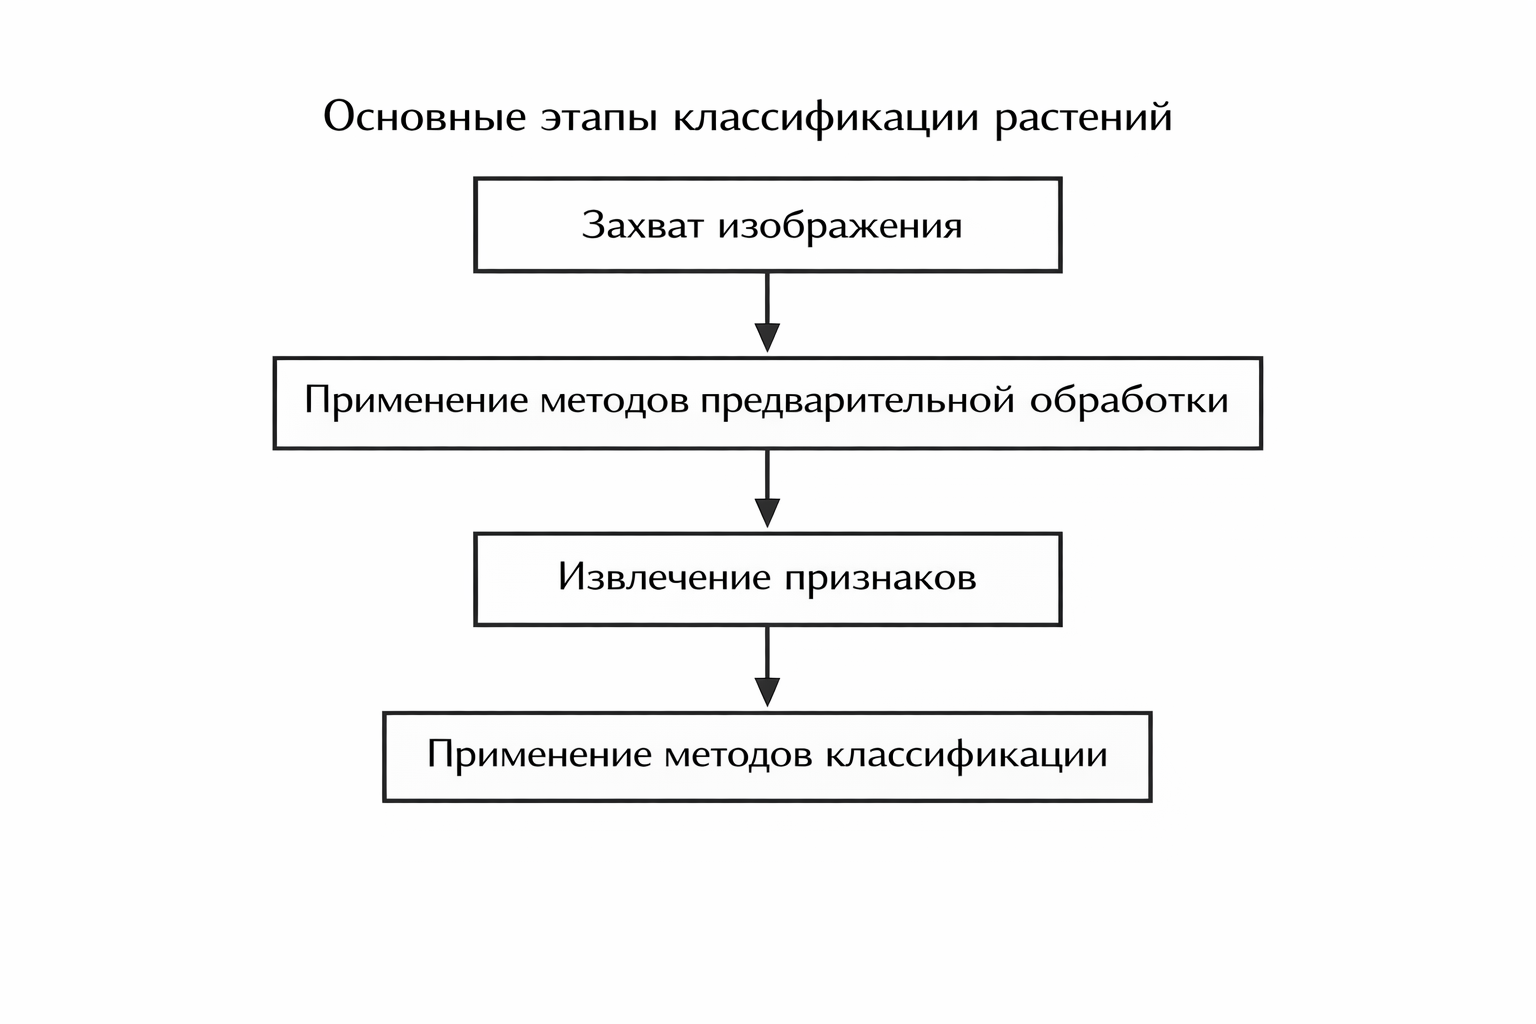
\includegraphics[width=\linewidth]{inc/img/general.png}
	\caption{Основные этапы классификации растений}
	\label{general}
\end{figure}
\clearpage
\section{Формализованная постновка задачи}
Функциональная модель представлена на рисунка~\ref{general_task}~-~\ref{details_task}.
\begin{figure}[h]
	\centering
	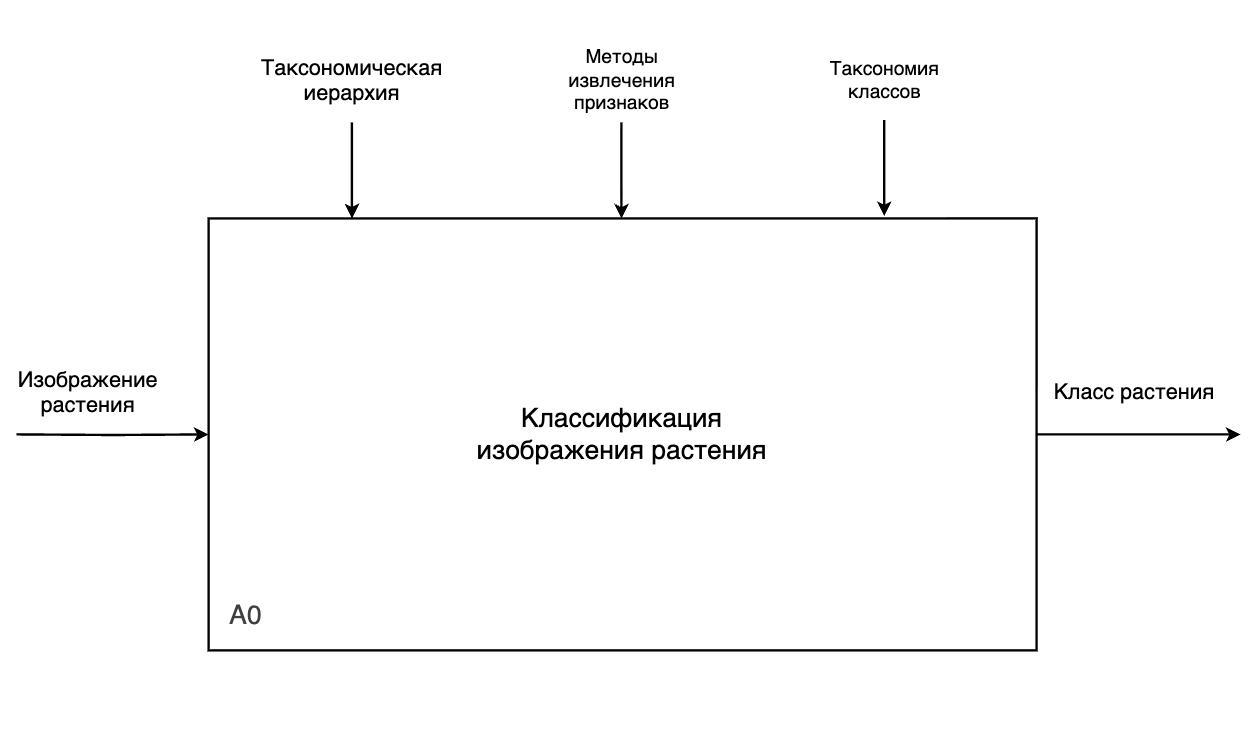
\includegraphics[width=0.7\linewidth]{inc/img/A0.png}
	\caption{Функциональная модель}
	\label{general_task}
\end{figure}

\begin{figure}[h]
	\centering
	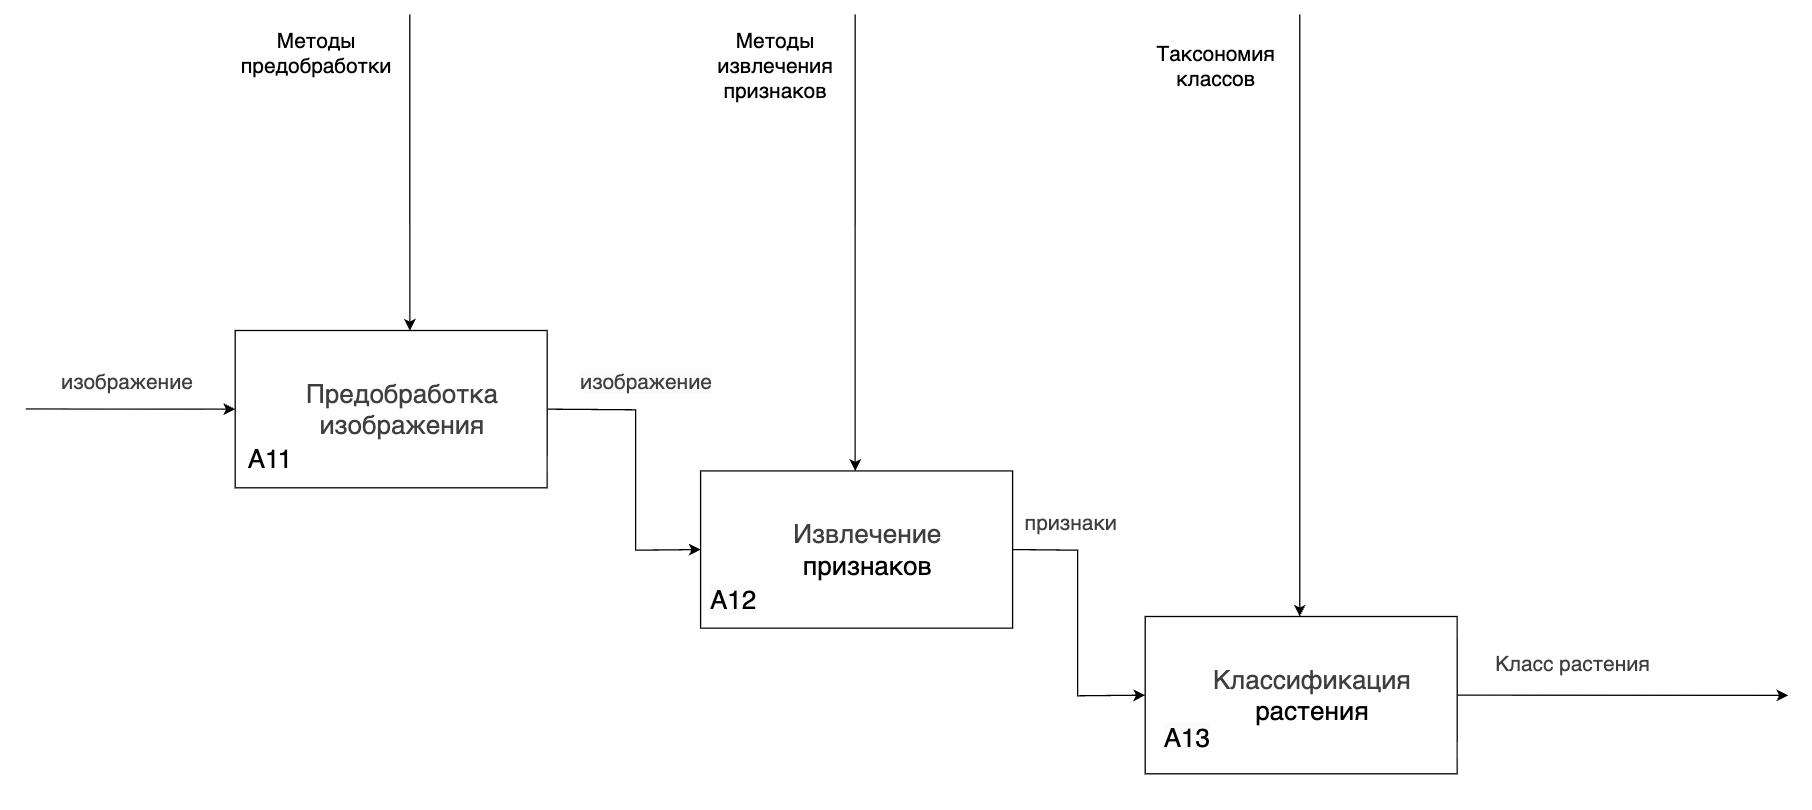
\includegraphics[width=\linewidth]{inc/img/A1.png}
	\caption{Функциональная модель}
	\label{details_task}
\end{figure}
\clearpage
%В качестве демонстрации общего подхода приведён псевдокод %для решения задачи классификации изображения на %листинге~\ref{example_algorithm}. 

%\begin{algorithm}[H]
%	\caption{Классификация изображений растений с использованием глубокого обучения}
%	\label{example_algorithm}
%	\begin{algorithmic}[1]
	%		\State \textbf{Вход:} обучающая выборка $X \in \mathbb{R}^{m \times n}$, метки классов $Y$, число слоёв $l$
	%		\State \textbf{Выход:} обученные веса модели или предсказанные метки классов
	%		\State Инициализировать веса модели малыми случайными значениями
	%		\State Задать скорость обучения $\alpha$, максимальное число эпох, порог ошибки
	%		\State Выполнить предварительную обработку данных: нормализация, изменение размера, one-hot кодирование меток
	%		\State Установить epoch $\leftarrow 0$, loss $\leftarrow \infty$
	%		\While{epoch $<$ max\_epochs и loss $>$ error\_threshold}
	%		\State epoch $\leftarrow$ epoch $+ 1$
	%		\For{всех мини-пакетов $(x_i, y_i)$ в обучающей выборке}
	%		\State \textbf{Прямой проход:}
	%		\State Пропустить входные данные $x_i$ через модель $f_{\theta}$ для получения предсказания $\hat{y}_i = f_{\theta}(x_i)$
	%		\State Модель $f_{\theta}$ может включать свёрточные слои, блоки внимания, нормализацию и нелинейности в зависимости от архитектуры
	%		\State Вычислить предсказание $\hat{y}_i$
	%		\State \textbf{Вычисление функции потерь:} вычислить $L(y_i, \hat{y}_i)$ (например, кросс-энтропию)
	%		\State \textbf{Обратное распространение ошибки:}
	%		\State Вычислить градиенты $\nabla_{\omega} L$
	%		\State Обновить веса: $\omega \leftarrow \omega - \alpha \cdot \nabla_{\omega} L$
	%		\EndFor
	%		\State Вычислить среднее значение функции потерь для текущей эпохи
	%		\State При необходимости выполнить оценку на валидационной или тестовой выборке
	%		\EndWhile
	%		\State \textbf{вернуть} обученную модель или предсказанные метки классов
	%	\end{algorithmic}
%\end{algorithm}
\section{Ограничения}
К ограничениям решения задачи относятся качество исходных изображений, и объем исходных данных, которые напрямую влияют на точность классификации, а также визуальная схожесть между растениями одного класса. 

Для сравнения методов используется датасет PlantClef 2015~\cite{ref1100}, поскольку данный датасет включает фотографии, собранные фотографами в разных точках мира, различных условиях. Вдобавок, данный датасет несбалансирован и имеет ограниченное количество изображений для некоторых видов, а также для него предопределен тестовый набор, что позволяет сравнивать методы, использующие данный датасет.


	\chapter{Методы решения задачи классификации изображений растения}
\section{Методы классификации на основе ручного извлечения признаков}
В данном разделе рассматриваются методы классификации изображений растений, основанные на ручном извлечении признаков и последующем применении алгоритмов машинного обучения. 
\textbf{Локальные бинарные паттерны}
Для заданного текстурного изображения LBP-код с параметрами $P$ и $R$, где $P$ равномерно расположенных пикселей выбираются на окружности радиуса $R$ относительно центрального пикселя, вычисляется для каждого пикселя изображения следующим образом:
\begin{equation}
	\mathrm{LBP}_{P,R} = \sum_{i=1}^{P} S \cdot 2^{i-1},
\end{equation}
где функция $S$ определяется как
\begin{equation}
	S =
	\begin{cases}
		1, & \text{если } (G_i - G_c) \geqslant 0, \\
		0, & \text{в противном случае}.
	\end{cases}
\end{equation}

Здесь $G_c$ и $G_i$ обозначают значения яркости центрального пикселя и соответствующего соседнего пикселя соответственно.

\clearpage
Пример взятия пикселей с различными заданными P, R приведён на рисунке~\ref{lbp_radious}.

\begin{figure}[h]
	\centering
	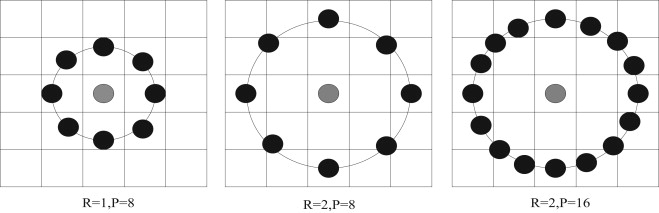
\includegraphics[width=\linewidth]{inc/img/lbp_radious.jpg}
	\caption{Схема выбора соседних пикселей в дескрипторе LBP для различных значений параметров $(P, R)$}
	\label{lbp_radious}
\end{figure}

В результате каждому пикселю изображения сопоставляется LBP-код, принимающий значения в диапазоне $[0, 2^{P} - 1]$. Далее всё изображение представляется в виде гистограммы, построенной по частотам появления LBP-кодов, вычисленных для всех пикселей изображения.

Базовый оператор LBP основан на жёстком пороговом сравнении, которое зависит от разности значений яркости центрального пикселя и соседнего пикселя. При этом возможно, что различные локальные пространственные структуры будут иметь одинаковый LBP-код, несмотря на различия в их геометрической организации. Это ограничивает дискриминативную способность базового LBP-дескриптора при различении сложных структурных паттернов~\cite{ref1000}.

Пример вычисления LBP-кода приведён на рисунке~\ref{lbp_example}
\begin{figure}[h]
	\centering
	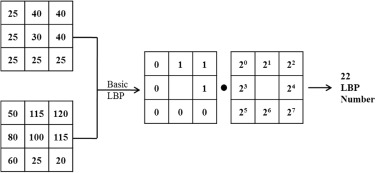
\includegraphics[width=\linewidth]{inc/img/lbp_example.jpg}
	\caption{Пример вычисления LBP-кода пикселя}
	\label{lbp_example}
\end{figure}
\clearpage

\textbf{Гистограмма ориентированных градиентов}

Метод базируется на анализе распределения направлений локальных градиентов яркости в плотной сетке и относится к классу плотных дескрипторов изображений.

Основная идея заключается в том, что локальный внешний вид и форма объекта могут быть эффективно охарактеризованы распределением направлений градиентов или границ, даже без точного знания их пространственного положения. На практике это реализуется путём разбиения изображения на небольшие пространственные области (ячейки), внутри которых накапливаются одномерные гистограммы направлений градиентов или ориентаций границ по всем пикселям соответствующей ячейки. Полученные значения гистограмм образуют вектор признаков.

Для повышения устойчивости к изменениям освещения, затенению и локальным изменениям контраста выполняется нормализация локальных откликов. Для этого энергия гистограмм аккумулируется в более крупных пространственных областях (блоках), после чего значения гистограмм всех ячеек, входящих в блок, нормализуются. Нормализованные блоки гистограмм образуют дескрипторы HOG.

Несмотря на успех разреженных признаков, таких как ключевые точки, плотное представление изображения в виде HOG-дескрипторов сохраняет высокую информативность и простоту, что делает его эффективным средством описания формы объектов.

Дескрипторы HOG обладают рядом преимуществ. Они эффективно захватывают структуру границ и градиентов, характерную для локальной формы объекта, и при этом обеспечивают контролируемую инвариантность к локальным геометрическим и фотометрическим преобразованиям. Небольшие смещения и повороты оказывают незначительное влияние на описание, если их масштаб меньше размера пространственных ячеек или угловых интервалов гистограммы.~\cite{ref1001}

Основные этапы реализации дескриптора HOG включают:
\begin{itemize}[label=---]
	\item вычисление градиентов изображения;
	\item построение гистограмм ориентаций для заданных областей;
	\item нормализацию гистограмм внутри сформированных групп областей.
\end{itemize}

Вычисление градиентов.
На первом этапе цветные текстурные изображения преобразуются в изображения в градациях серого. Горизонтальный градиент $f_a$ и вертикальный градиент $f_b$ вычисляются с использованием дифференцирующих масок для изображения в градациях серого. Применение более сложных масок снижает производительность системы, поэтому используется простая дифференцирующая маска. Горизонтальный $f_a$ и вертикальный $f_b$ градиенты изображения вычисляются следующим образом:
\begin{equation}
	f_a(a,b) = I(a+1,b) - I(a-1,b),
\end{equation}
\begin{equation}
	f_b(a,b) = I(a,b+1) - I(a,b-1),
\end{equation}
где $I(a,b)$ представляет значение интенсивности пикселя в точке $(a,b)$.

Построение гистограмм ориентаций.
С использованием горизонтального $f_a$ и вертикального $f_b$ градиентов изображения вычисляются величина градиента $m$ и ориентация градиента $\theta$ следующим образом:
\begin{equation}
	m(a,b) = \sqrt{f_a(a,b)^2 + f_b(a,b)^2},
\end{equation}
\begin{equation}
	\theta(a,b) = \tan^{-1}\left(\frac{f_b(a,b)}{f_a(a,b)}\right).
\end{equation}

Направленная гистограмма градиентов.
На практике ориентации градиента, меньшие нуля, суммируются с $180^\circ$, поскольку требуемые значения направлений должны быть немаркированными. Соответственно, немаркированные ориентации градиентов нового изображения вычисляются следующим образом:
\begin{equation}
	\tilde{\theta}(a,b) =
	\begin{cases}
		\theta(a,b) + \pi, & \text{если } \theta(a,b) < 0, \\
		\theta(a,b), & \text{в противном случае}.
	\end{cases}
\end{equation}

После вычисления ориентаций градиентов изображение разбивается на ячейки фиксированного размера $[u \times v]$ пикселей. Угол ориентации $\tilde{\theta}(a,b)$ распределяется по соответствующему угловому интервалу для формирования гистограммы ориентаций каждой ячейки. Гистограмма ориентаций формируется путём равномерного разбиения диапазона $0^\circ$--$180^\circ$

Нормализация по блокам.
Блочная нормализация отображает гистограммы ориентаций для каждой ячейки с вычитанием больших блоков размером $[n \times m]$. Поскольку каждая ячейка содержит $k$ ориентаций, размер вектора признаков для каждого блока составляет $[n \times m \times k]$. Вектор признаков $\mathbf{v}$ представляет ненормализованную гистограмму в точке $(i,j)$ блока $p(i,j)$. Нормализация вектора признаков выполняется с использованием $L_2$-нормы следующим образом
\begin{equation}
	\mathbf{v}' = \frac{\mathbf{v}}{\sqrt{\|\mathbf{v}\|^2 + \varepsilon}}
\end{equation}
где $\varepsilon$~---~малая нормализующая константа, используемая для предотвращения деления на ноль.

Иллюстрация получения гистограммы для ячейки представлен на изображении~\ref{hog_example}

\begin{figure}[h]
	\centering
	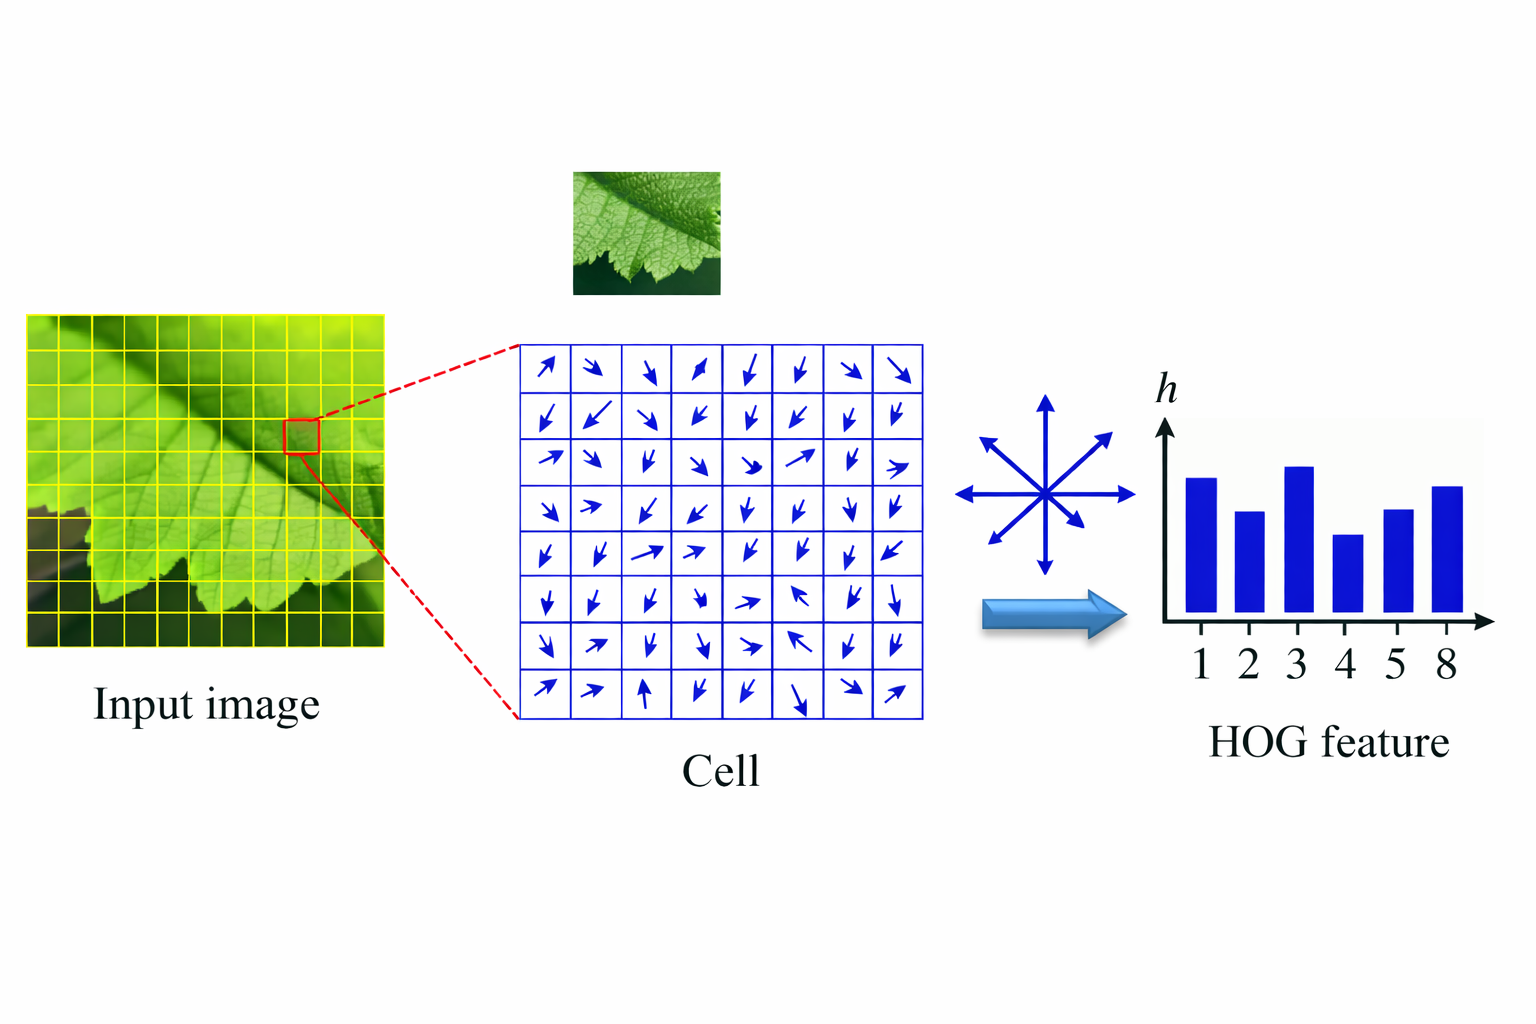
\includegraphics[width=\linewidth]{inc/img/hog_example.png}
	\caption{Иллюстрация получения гистограммы для ячейки}
	\label{hog_example}
\end{figure}
\clearpage

\textbf{Метод k-ближайших соседей}


Метод $k$-ближайших соседей (kNN) является алгоритмом машинного обучения с учителем, первоначально разработанным Эвелин Фикс и Джозефом Ходжесом в 1951 году и впоследствии усовершенствованным Томасом Ковером.

Алгоритм $k$-ближайших соседей (kNN) относится к непараметрическим методам обучения на экземплярах и широко используется в задачах обучения с учителем, включая классификацию и регрессию. В отличие от модельно-ориентированных методов, которые строят явную функцию на основе обучающей выборки, алгоритм kNN относится к классу ленивых алгоритмов обучения. Он не требует предварительного этапа обучения и формирует прогнозы непосредственно при появлении нового объекта, анализируя структуру данных в пространстве признаков. Принцип работы kNN основан на предположении о сходстве данных, согласно которому похожие объекты, как правило, располагаются близко друг к другу в пространстве. Следовательно, прогноз для нового объекта определяется на основе его близости к существующим объектам обучающей выборки.

\textbf{Основные этапы алгоритма kNN.}

\begin{enumerate}
	\item \textbf{Выбор параметра $k$.}  
	На первом этапе выбирается число ближайших соседей $k$, которое является ключевым гиперпараметром алгоритма и подбирается с учётом характеристик конкретного набора данных. Значение $k$ существенно влияет на точность классификации: малые значения $k$ повышают чувствительность к шуму и могут приводить к переобучению, тогда как большие значения $k$ увеличивают вычислительные затраты и могут вызывать недообучение.
	
	\item \textbf{Вычисление расстояний.}  
	Для нового объекта вычисляется расстояние до всех объектов обучающей выборки. Наиболее распространёнными метриками расстояния являются евклидова, манхэттенская и метрика Минковского. Выбор метрики расстояния оказывает значительное влияние на качество работы алгоритма и должен учитывать свойства пространства признаков.
	
	\item \textbf{Определение ближайших соседей.}  
	Все объекты обучающей выборки упорядочиваются по возрастанию расстояния до нового объекта, после чего выбираются $k$ ближайших соседей.
	
	\item \textbf{Агрегация ответов соседей.}  
	В задачах классификации класс нового объекта определяется по принципу большинства голосов среди $k$ ближайших соседей. В задачах регрессии прогнозируемое значение может быть вычислено как среднее или медианное значение целевой переменной соседних объектов.
\end{enumerate}

\textbf{Выбор параметров и его влияние на работу алгоритма:}


Выбор значения $k$ оказывает существенное влияние на поведение модели. Малые значения $k$ могут приводить к переобучению, поскольку алгоритм начинает учитывать шумовые особенности данных. Напротив, большие значения $k$ сглаживают границу принятия решений, что может приводить к потере важной структуры данных и недообучению модели.

Выбор метрики расстояния также является критически важным. Хотя евклидово расстояние используется наиболее часто, альтернативные метрики, такие как манхэттенская или метрика Минковского, могут быть более подходящими при работе с высокоразмерными данными или в случаях, когда требуется различная чувствительность к отдельным признакам.

\textbf{Проблемы алгоритма kNN.}

Современные исследования, посвящённые алгоритму $k$-ближайших соседей, выделяют ряд ключевых проблем.

\begin{enumerate}
	\item Выбор оптимального значения $k$.
	Определение наиболее подходящего числа соседей остаётся сложной задачей, поскольку данный параметр напрямую влияет на точность и обобщающую способность алгоритма.
	
	\item Вычислительная сложность. 
	Классическая реализация kNN требует значительных вычислительных ресурсов при работе с большими наборами данных, так как для каждого нового объекта необходимо вычислять расстояния до всех элементов обучающей выборки.
	
	\item Работа с высокоразмерными данными.
	Эффективность алгоритма kNN снижается в пространствах высокой размерности вследствие эффекта <<проклятия размерности>>, при котором расстояния между объектами теряют информативность.
	
	\item Чувствительность к шуму и выбросам.
	Зависимость алгоритма от ближайших соседей делает его уязвимым к шумовым данным и выбросам, что может негативно сказываться на качестве классификации.
\end{enumerate}

\clearpage

\textbf{Метод опорных векторов}


Метод опорных векторов (Support Vector Machine, SVM) является одним из широко используемых алгоритмов обучения с учителем, применяемых для решения задач классификации и регрессии. В основе метода лежит идея построения оптимальной разделяющей гиперплоскости в пространстве признаков, которая обеспечивает максимальный зазор между объектами различных классов. Такой подход позволяет повысить обобщающую способность классификатора и снизить риск переобучения.

Пусть обучающая выборка задана в виде набора пар $(\mathbf{x}_i, y_i)$, где $\mathbf{x}_i \in \mathbb{R}^d$~---~вектор признаков объекта, а $y_i \in \{-1, +1\}$~---~соответствующая метка класса. В линейно разделимом случае задача SVM заключается в нахождении такой гиперплоскости
\[
\mathbf{w}^T \mathbf{x} + b = 0,
\]
которая разделяет классы и максимизирует расстояние от ближайших объектов обучающей выборки до этой гиперплоскости. Объекты, находящиеся на границе зазора, называются опорными векторами и именно они определяют положение разделяющей поверхности.

Для реальных данных, которые, как правило, не являются строго линейно разделимыми, в методе SVM используется концепция мягкого зазора (soft margin). В этом случае допускаются ошибки классификации, величина которых контролируется с помощью параметра штрафа $C$. Данный параметр задаёт компромисс между шириной зазора и количеством ошибок на обучающей выборке: большие значения $C$ приводят к более строгому разделению классов, тогда как меньшие значения повышают устойчивость модели к шуму.

Для решения задач нелинейной классификации в SVM применяется так называемый ядерный трюк (kernel trick), позволяющий неявно отображать исходные данные в пространство большей размерности, где они могут стать линейно разделимыми. Вместо явного вычисления отображения используется ядерная функция
\[
K(\mathbf{x}_i, \mathbf{x}_j) = \langle \phi(\mathbf{x}_i), \phi(\mathbf{x}_j) \rangle,
\]
которая вычисляет скалярное произведение в новом пространстве признаков. На практике широко применяются линейное, полиномиальное и гауссово (RBF) ядра. Выбор ядра и его параметров существенно влияет на качество классификации и определяется характеристиками конкретной задачи.

Благодаря способности эффективно работать в пространствах высокой размерности и устойчивости к переобучению метод опорных векторов широко используется в задачах анализа изображений, в том числе для классификации объектов на основе заранее извлечённых признаков, таких как LBP и HOG.

\clearpage

	\section{\texorpdfstring{Методы \mbox{классификации} с \mbox{использованием} \mbox{свёрточных} \mbox{нейронных} \mbox{сетей}}{Методы классификации с использованием свёрточных нейронных сетей}}
\textbf{Принцип работы свёрточных нейронных сетей}

Свёрточная нейронная сеть (Convolutional Neural Network, CNN) является типом модели глубокого обучения, предназначенной для обработки данных, имеющих решётчатую структуру, таких как изображения.

CNN представляет собой математическую модель, которая, как правило, состоит из трёх основных типов слоёв: свёрточных слоёв, слоёв подвыборки (pooling) и полносвязных слоёв. Свёрточные и pooling-слои используются для извлечения признаков, тогда как полносвязные слои выполняют отображение извлечённых признаков в выходные значения, например в классы при классификации изображений.

Свёрточный слой является ключевым компонентом архитектуры CNN и состоит из набора математических операций, включая свёртку~---~специализированный тип линейной операции. В цифровых изображениях значения пикселей хранятся в виде двумерной сетки чисел, и массив обучаемых параметров, называемый ядром, применяется ко всем локальным областям изображения. Благодаря этому CNN особенно эффективны для анализа изображений, поскольку один и тот же признак может появляться в различных частях изображения.

По мере прохождения данных через последовательные слои сети извлекаемые признаки становятся иерархически более сложными. Процесс настройки параметров сети, таких как ядра свёрточных слоёв и веса полносвязных слоёв, называется обучением и выполняется с целью минимизации различия между выходными предсказаниями сети и истинными метками обучающих данных.

В отличие от традиционных методов анализа изображений, где признаки извлекаются вручную, CNN позволяют автоматически извлекать признаки непосредственно из исходных изображений. Кроме того, архитектуры CNN, как правило, не требуют предварительной сегментации объектов, выполняемой экспертами, что снижает зависимость качества модели от субъективных факторов. Однако CNN содержат большое количество обучаемых параметров, что требует значительных вычислительных ресурсов и наличия достаточно больших наборов обучающих данных. Для эффективного обучения CNN обычно используются графические процессоры (GPU).

Архитектура CNN включает свёрточные слои, pooling-слои и полносвязные слои. Типичная архитектура состоит из повторяющихся блоков, включающих один или несколько свёрточных слоёв и слой подвыборки, за которыми следуют полносвязные слои. Процесс преобразования входных данных в выходные значения посредством последовательного прохождения через слои сети называется прямым распространением (forward propagation).

\textbf{Свёрточный слой}


Свёрточный слой выполняет извлечение признаков и является фундаментальным элементом CNN. Он состоит из линейной операции свёртки, за которой следует нелинейная функция активации.

\textbf{Операция свёртки}


Свёртка представляет собой специализированный тип линейной операции, при которой массив чисел, называемый ядром, применяется к входному тензору. В каждой позиции выполняется поэлементное произведение элементов ядра и соответствующих элементов входного тензора, результаты которого суммируются для получения значения в выходной карте признаков.

Применение нескольких ядер позволяет формировать несколько карт признаков, каждая из которых отражает различные характеристики входных данных. Таким образом, различные ядра могут рассматриваться как отдельные извлекатели признаков.

Основными гиперпараметрами операции свёртки являются размер ядра и их количество, что определяет глубину выходных карт признаков.

Поскольку стандартная операция свёртки приводит к уменьшению пространственных размеров выходного тензора, часто применяется метод дополнения, при котором по краям входного тензора добавляются нулевые значения. Это позволяет сохранить пространственные размеры карт признаков.

Ключевой особенностью операции свёртки является совместное использование весов, при котором одно и то же ядро применяется ко всем позициям изображения. Это обеспечивает инвариантность к сдвигу, формирование иерархий признаков и уменьшение числа обучаемых параметров по сравнению с полносвязными сетями.

\textbf{Функция активации}


После линейной операции свёртки применяется нелинейная функция активации. В современных CNN наиболее распространённой функцией активации является выпрямленная линейная единица (Rectified Linear Unit, ReLU), определяемая как $\max(0, x)$.

\textbf{Pooling-слой}


Pooling-слой используется для понижения пространственной размерности карт признаков и повышения устойчивости модели к небольшим сдвигам и искажениям. В pooling-слоях отсутствуют обучаемые параметры, однако размер фильтра, шаг и способ подвыборки задаются как гиперпараметры.

\textbf{Max-pooling}


Max-pooling является наиболее распространённой pooling-операцией, при которой из каждого локального фрагмента карты признаков выбирается максимальное значение. Обычно используется фильтр размером $2 \times 2$ с шагом 2, что уменьшает высоту и ширину карты признаков в два раза.

\textbf{Глобальный average-pooling}


Глобальный average-pooling преобразует карту признаков в тензор размером $1 \times 1$ путём усреднения всех значений. Эта операция позволяет уменьшить количество параметров модели и обеспечивает возможность обработки входных изображений переменного размера.

\textbf{Полносвязные слои}


Выходные карты признаков последнего свёрточного или pooling-слоя преобразуются в одномерный вектор и подаются на вход одного или нескольких полносвязных слоёв. Эти слои выполняют отображение извлечённых признаков в выходное пространство, например в вероятности классов.

Для задач многоклассовой классификации в последнем слое обычно используется функция активации softmax, которая нормализует выходные значения в вероятности, сумма которых равна единице.

\textbf{Обучение и функция потерь}


Обучение CNN заключается в настройке параметров сети~---~ядер свёрточных слоёв и весов полносвязных слоёв~---~таким образом, чтобы минимизировать функцию потерь, измеряющую расхождение между предсказаниями сети и истинными метками обучающих данных.

Функция потерь выбирается в зависимости от решаемой задачи. Для задач классификации обычно используется перекрёстная энтропия, тогда как для задач регрессии применяется среднеквадратичная ошибка.

Градиентный спуск обычно используется в качестве алгоритма оптимизации, который итеративно обновляет обучаемые параметры сети, то есть ядра и веса, с целью минимизации функции потерь.

\textbf{Примеры моделей CNN}

\textbf{AlexNet}

Архитектура AlexNet была предложена Алексом Крижевским и Джеффри Хинтоном. Архитектура сети, использованная в данной работе, представлена на рис.~\ref{arch_alex}. Сеть AlexNet содержит восемь взвешенных слоёв, первые пять из которых являются свёрточными слоями, а оставшиеся три~---~полностью связанными слоями.

За первыми двумя свёрточными слоями следуют слои нормализации и пулинга. После последнего свёрточного слоя располагается один слой пулинга. Третий, четвёртый и пятый свёрточные слои соединены напрямую. Второй полностью связанный слой передаёт данные классификатору softmax, который формирует вероятности принадлежности к классам.

В качестве функции активации в первых двух полностью связанных слоях (fc6 и fc7) используется функция ReLU, которая генерирует 4096 значений. Выход седьмого слоя, содержащий 4096 элементов, полностью соединён с нейронами восьмого слоя (fc8), где число нейронов соответствует количеству классов. После обучения выходной слой fc8 формирует значения с плавающей запятой, представляющие прогнозируемый результат классификации.

\begin{figure}[h]
	\centering
	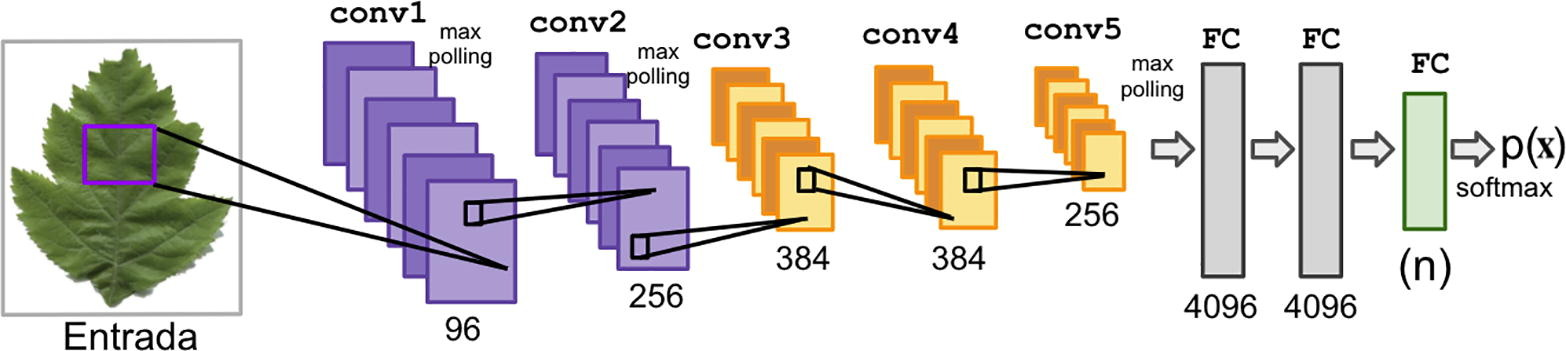
\includegraphics[width=\linewidth]{inc/img/arch_alex.jpg}
	\caption{Архитектура AlexNet}
	\label{arch_alex}
\end{figure}

\textbf{GoogLeNet}


Архитектура GoogLeNet стала победителем конкурса ILSVRC 2014 года, продемонстрировав ошибку 6{,}67\% по метрике top-5. Данная архитектура показала высокую эффективность при решении задач, характеризующихся высокой сложностью, достигнув высокой точности при относительно низкой вычислительной нагрузке.

В отличие от AlexNet, GoogLeNet реализует иной подход к построению сети и включает в себя специализированные структурные элементы, называемые модулями inception. Общая структура архитектуры GoogLeNet представлена на рис.~\ref{arch_google}. Модуль inception использует переменные рецептивные поля, сформированные с помощью свёрточных ядер различного размера. Это позволяет эффективно фиксировать редкие корреляционные паттерны в картах признаков.

Архитектура GoogLeNet состоит из 22 слоёв, что существенно превышало глубину ранее предложенных сетей. При этом количество параметров в GoogLeNet значительно меньше и составляет примерно одну двенадцатую от числа параметров AlexNet. В архитектуре используются девять модулей inception (M1--M9). Основная идея inception заключается в локализации оптимальной разреженной структуры и её аппроксимации плотным представлением.

Каждый модуль inception включает несколько свёрток с ядрами размером $1\times1$, $3\times3$ и $5\times5$, а также слой max-pooling, результаты которых объединяются. Такой подход отличает GoogLeNet от традиционной многоканальной свёртки. Для снижения вычислительной сложности и предотвращения переобучения применяются стратегии усредняющего пулинга и отсева после модулей inception, что способствует уменьшению размерности признакового пространства. Более подробное описание данной архитектуры приведено в~\cite{ref40}.

\begin{figure}[h]
	\centering
	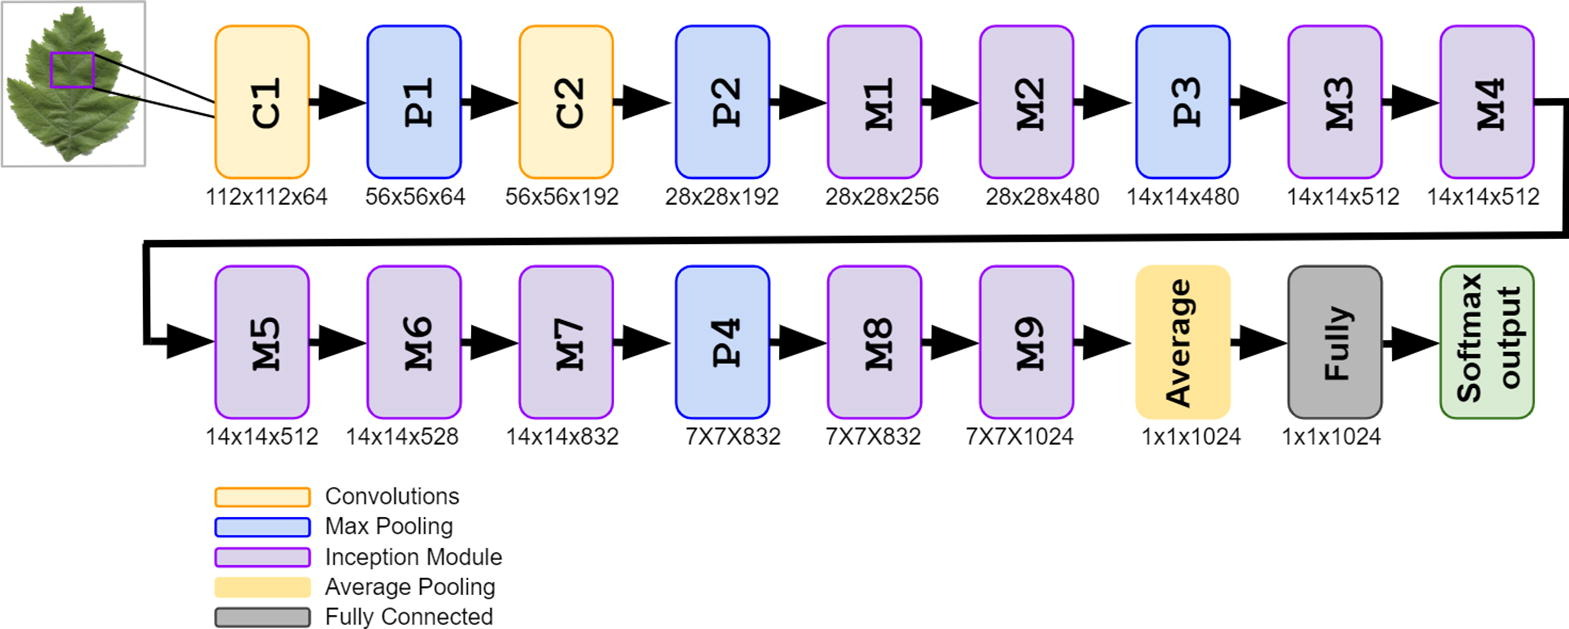
\includegraphics[width=\linewidth]{inc/img/arch_google.jpg}
	\caption{Архитектура GoogLeNet}
	\label{arch_google}
\end{figure}

\textbf{VGGNet}


Архитектура VGGNet была разработана Кареном Симоняном и Эндрю Зиссерманом и заняла второе место в конкурсе ILSVRC 2014 года. VGGNet представляет собой развитие идей, заложенных в архитектуре AlexNet. Структура сети показана на рис.~\ref{arch_vgg}.

Основной особенностью VGGNet является использование исключительно свёрточных ядер размером $3\times3$ и слоёв максимального пулинга размером $2\times2$. Архитектура VGG включает пять блоков свёрточных слоёв, каждый из которых завершается слоем максимального пулинга. После свёрточных блоков следуют два полностью связанных слоя и выходной слой.

Первые два блока содержат по два свёрточных слоя с 64 и 128 фильтрами соответственно. Следующие два блока включают по три свёрточных слоя с 256, 512 и 512 фильтрами. Все слои максимального пулинга имеют размер окна $2\times2$ и шаг, равный 2.

VGGNet является одной из наиболее популярных архитектур в литературе для извлечения признаков из изображений. Однако данная архитектура содержит около 138 миллионов параметров, что может затруднять её практическое использование. В литературе широко представлены модификации VGGNet, такие как VGG16 и VGG19. В данной работе использовалась архитектура VGG16, состоящая из 16 глубоких свёрточных слоёв.

\begin{figure}[h]
	\centering
	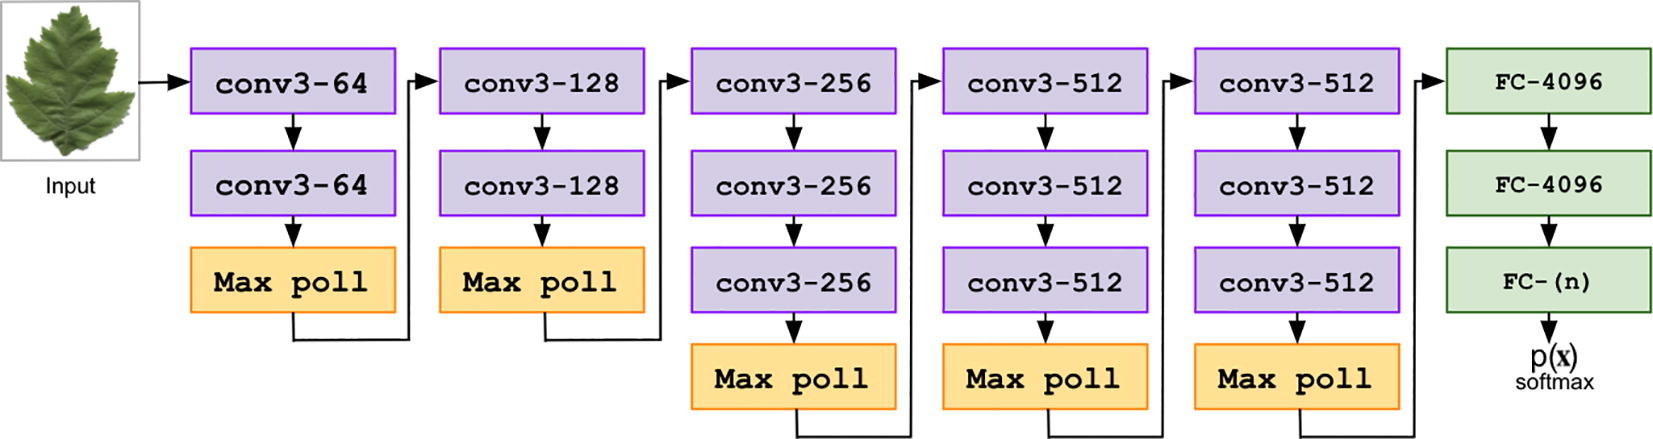
\includegraphics[width=\linewidth]{inc/img/arch_vgg.jpg}
	\caption{Архитектура VGGNet}
	\label{arch_vgg}
\end{figure}
\textbf{FGIC-классификация}

В методах FGIC (fine-grained image classification) распознавание проводится по иерархии классов. Для растений такая иерархия естественным образом задаётся ботанической таксономией, включающей уровни семейства, рода и вида. Эксперты-ботаники традиционно используют именно такой подход, определяя род растения и уточняя конкретный вид~\cite{ref35}. 

Иерархический подход снижает сложность классификации за счёт поэтапного уточнения решения: на первом этапе производится грубая классификация по более общим таксономическим категориям, после чего выполняется детальная классификация внутри ограниченного подмножества классов. Такой подход позволяет сгруппировать визуально схожие объекты и тем самым уменьшить влияние межклассовых и внутриклассовых вариаций.

Различия между близкими видами характеризуются низкой вариативностью формы и цвета, поэтому при детальной классификации используется локальное представление изображения листа.

\textbf{Сиамские нейронные сети}

Сиамские нейронные сети (SCNN) представляют собой нейронные сети, состоящие из двух или более симметричных (идентичных) подсетей. Ключевым признаком, позволяющим отнести сеть к классу сиамских, является совместное использование весов между идентичными подсетями~\cite{ref78}. Сиамская сеть функционирует следующим образом: входные данные подаются параллельно во все идентичные подсети, после чего производится сравнение выходных представлений, и на основе этого сравнения принимается решение о принадлежности входных данных (изображения) к тому или иному классу~\cite{ref79}.

SCNN имеет схожую структуру с CNN, включая свёрточные и pooling-слои, однако в ней отсутствует слой softmax. В отличие от обычных CNN, разность выходов полносвязных слоёв передаётся на один нейрон с монотонной функцией активации (чаще всего сигмоидной), формирующей бинарный выход (0 или 1). Общая архитектура сиамской нейронной сети показана на рис.~\ref{scnn_example}

\begin{figure}[h]
	\centering
	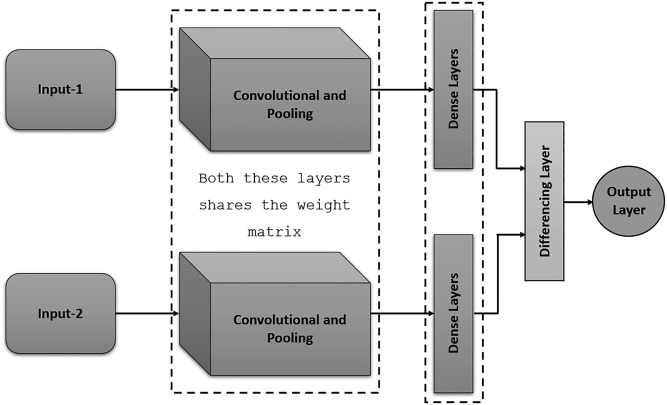
\includegraphics[width=\linewidth]{inc/img/SCNN_example.jpg}
	\caption{Архитектура SCNN}
	\label{scnn_example}
\end{figure}
\textbf{Гибридные подходы}

В работе "On the Behavior of Convolutional Nets for Feature Extraction"~\cite{ref1006} показано, что обученные CNN способны извлекать визуальные дескрипторы, которые можно использовать в задачах, отличных от исходной задачи обучения сети, без необходимости дорогостоящей фазы обучения на целевых данных. Применение такого подхода обычно заключается в извлечении признаков из слоёв сети, близких к выходу, и последующей подаче этих признаков в классический классификатор, что обеспечивает устойчивую и информативную характеристику изображений~\cite{ref1006}. Извлечённые признаки могут использоваться в других задачах машинного обучения, включая классификацию, кластеризацию или оценку сходства, без повторного обучения самой сети.

В работе "Two-view fine-grained classification of plant species"~\cite{ref1007} авторы предлагают использование иерархического подхода с глобальным и локальным представлением листа, используя SCNN в качестве основной архитектуры, поскольку одной из главных задач является классификация визуально схожих видов общего рода при малом количестве данных. Благодаря использованию SCNN не требуется переобучения при добавлении новых видов, поскольку результатом работы является не класс, а сходство между тестовым и эталонными изображениями. Предложенный подход иллюстрируется на рис.~\ref{super_example}.

\begin{figure}[h]
	\centering
	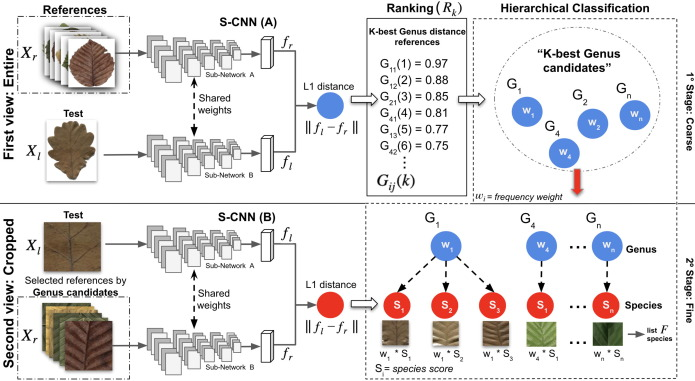
\includegraphics[width=\linewidth]{inc/img/super_example.jpg}
	\caption{Иерархическая классификация с использованием SCNN}
	\label{super_example}
\end{figure}

\section{Сравнительный анализ подходов}

Для анализа применимости рассмотренных подходов к задаче тонкозернистой классификации изображений растений вводится совокупность критериев, охватывающих как количественные характеристики качества классификации, так и концептуальные свойства методов.

Введены следующие критерии сравнения:
\begin{enumerate}
	\item тип используемых признаков;
	\item требуется ли повторное обучение при добавлении новых классов;
	\item зависимость качества от объёма размеченных данных;
	\item вычислительная сложность обучения;
	\item вычислительная сложность инференса;
	\item интерпретируемость используемых признаков;
	\item применимость к задачам тонкозернистой классификации изображений.
\end{enumerate}

На основе введённых критериев составлена сравнительная таблица~\ref{criteries_table}, позволяющая проанализировать сильные и слабые стороны рассмотренных подходов в контексте задачи классификации изображений растений.

\begin{table}[h]
	\centering
	\caption{Сравнение подходов к классификации изображений растений по строгим критериям}
	\label{criteries_table}
	\renewcommand{\arraystretch}{1.2}
	\resizebox{\linewidth}{!}{%
		\begin{tabular}{|p{5.2cm}|c|c|c|c|c|}
			\hline
			\textbf{Критерий / подход} & \textbf{\begin{tabular}[c]{@{}c@{}}LBP/HOG\\+ kNN/SVM\end{tabular}} & \textbf{\begin{tabular}[c]{@{}c@{}}CNN\\end-to-end\end{tabular}} & \textbf{\begin{tabular}[c]{@{}c@{}}CNN как\\экстрактор\end{tabular}} & \textbf{\begin{tabular}[c]{@{}c@{}}Siamese\\CNN\end{tabular}} & \textbf{\begin{tabular}[c]{@{}c@{}}Комбинированный\\\end{tabular}} \\
			\hline
			Тип признаков & ручные & обучаемые & обучаемые & обучаемые & обучаемые \\
			\hline
			Требуется повторное обучение при добавлении новых классов & нет$^{*}$ & да & нет$^{**}$ & нет$^{**}$ & нет$^{**}$ \\
			\hline
			Зависимость качества от объёма размеченных данных & высокая & высокая & средняя & ниже & ниже \\
			\hline
			Вычислительная сложность обучения & низкая & высокая & низкая--средняя & высокая & высокая \\
			\hline
			Вычислительная сложность инференса & низкая & средняя & средняя & высокая & высокая \\
			\hline
			Интерпретируемость используемых признаков & высокая & низкая & низкая & низкая & низкая \\
			\hline
			Типичная область применимости в FGIC & ограниченно & да & да & да & да \\
			\hline
	\end{tabular}}
	\vspace{2mm}
	
	{\footnotesize $^{*}$ Добавление нового класса возможно без переобучения при условии переразметки/донастройки классификатора и наличия признаков для новых образцов. \\
		$^{**}$ Добавление нового класса возможно путём добавления эталонных образцов (reference images) без изменения весов модели при метрической постановке задачи.}
\end{table}

	\chapter*{ЗАКЛЮЧЕНИЕ}
\addcontentsline{toc}{chapter}{ЗАКЛЮЧЕНИЕ}

В ходе выполнения выпускной квалификационной работы была достигнута поставленная цель~---~разработан метод классификации растений по изображениям листьев с использованием свёрточной нейронной сети.

Для достижения цели были решены следующие задачи:
\begin{enumerate}[itemsep=0pt, parsep=0pt, topsep=0pt]
	\item проведён анализ предметной области с целью выявления проблем в задачах таксономизации растений;
	\item формализована задача для проведения классификации изображений листьев растений средней полосы России;
	\item разработан двухэтапный метод классификации растений по изображениям листьев с использованием свёрточной нейронной сети;
	\item разработаны алгоритмы для реализации предложенного метода;
	\item реализована программа на основе разработанного метода;
	\item выполнено сравнение результатов расчётов по разработанному методу с результатами классификации после прямого обучения.
\end{enumerate}

Разработанный метод реализован в виде программного приложения, поддерживающего загрузку изображений, формирование эталонного индекса и получение ранжированного списка наиболее вероятных видов растений. Проведённые исследования показали применимость предложенного подхода для задачи классификации растений по изображениям листьев.


	\printbibliography[
	heading=bibintoc,
	title={СПИСОК ИСПОЛЬЗОВАННЫХ ИСТОЧНИКОВ}
	]

	%\begin{appendices}[А]
%	\chapter{}
	
%\end{appendices}

\chapter*{ПРИЛОЖЕНИЕ А}
\addcontentsline{toc}{chapter}{ПРИЛОЖЕНИЕ А} % добавляем в оглавление
\phantomsection % чтобы hyperref корректно сделал ссылку
Презентация к выпускной квалификационной работе на тему <<Классификация изображений растений>> состоит из 3 слайдов.


\end{document}
